\documentclass{bredelebeamer}

%%%%%%%%%%%%%%%%%%%%%%%%%%%%%%%%%%%%%%%%%%%%%%%%

\title[Programación en MatLAB]{Introducción a la programación con MatLAB}
\subtitle{Módulo 10 - Álgebra matricial}

\author{Autor1 - Autor2 - Autor3\inst{1}}
\institute[UTN.BA]
{
  \inst{1}%
  Universidad Tecnológica Nacional\\
  Facultad Regional Buenos Aires
  }

\date{dia mes 2018}

\subject{Taller de programación}

\logo{

\includegraphics[scale=0.15]{images/logo.png}
}

%%%%%%%%%%%%%%%%%%%%%%%%%%%%%%%%%%%%%%%%%%%%%%%%%%%%%%%%%%%%%%%%%%%%%
\begin{document}

\begin{frame}
  \titlepage 
\end{frame}

%%%%%%%%%%%%%%%%%%%%%%%%%%%%%%%%%%%%%%%%%%%%%%%%%%%%%%%%%%%%%%%%%%%%%

% Algebra matricial

%%%%%%%%%%%%%%%%%%%%%%%%%%%%%%%%%%%%%%%%%%%%%%%%%%%%%%%%%%%%%%%%%%%%%
\section{Algebra matricial}

\begin{frame}{Transpuesta}
El operador \textbf{transpose} (transpuesta) cambia las filas de una matriz en culumnas y las columnas en fila. En matlab el operador transpuesta se define como:
\begin{center}
Transpuesta\_A = A'
\end{center}
Ej. Ejecutar las siguientes líneas. Obtener conclusiones.
\boiteviolette{
A = [1 2 3 4 5 6];\\
A'\\
B = [1 2 3 ; 4 5 6 ; 7 8 9];\\
B'
}
\end{frame}

\begin{frame}{Producto punto}
El producto punto (producto escalar) se define como:
\begin{center}
Vector\_resultante = sum(A\textbf{.*}B)
\end{center}
Ej. Ejecutar las siguientes líneas. Obtener conclusiones.
\boiteviolette{
A = [1 2 3 4 5];\\
B = [2 3 4 5 6];\\
sum(A.*B)
}
\begin{exampleblock}{Comando}
Ver comando: dot()
\end{exampleblock}
Ej. Ejecutar las siguientes líneas. Obtener conclusiones.
\boiteviolette{
A = [1 2 3 4 5];\\
B = [2 3 4 5 6];\\
dot(A,B)
}
\end{frame}

\begin{frame}{Ejercicio práctico xxx}
\begin{enumerate}
\item Use la función dot para encontrar el producto punto de los siguientes vectores:
\begin{itemize}
\item A = [1 2 3 4]
\item B = [12 20 15 7]
\end{itemize}
\item Encuentre el producto punto de A y B al sumar los productos arreglo de A y B (sum(A.*B))
\end{enumerate}
\end{frame}

\begin{frame}{Multiplicación matricial}
El producto matricial se realiza utilizando el operador \textbf{*}
\begin{center}
Vector\_resultante = A*B
\end{center}
\boiteviolette{
A = [1 2 3 4 5];\\
B = [2 3 4 5 6];\\
VectorResultante = A*B
}
\end{frame}

\begin{frame}{Potencias de matrices}
Elevar a la potencia N cada elemento de la matriz se define mediante el operador \textbf{.\^}
\begin{center}
Vector\_resultante = A.\^N
\end{center}
\boiteviolette{
A = [1 2 3 4 5];\\
B = 2;\\
VectorResultante = A.\^B
}
Elevar a la potencia N  la matriz se define mediante el operador \textbf{\^}
\begin{center}
Vector\_resultante = A\^N
\end{center}
\boiteviolette{
A = [1 2 3 4 5];\\
B = 2;\\
VectorResultante = A\^B
}
\end{frame}

\begin{frame}{Inversión de matriz}
\begin{exampleblock}{Comando}
Ver comando: inv()
\end{exampleblock}
Ej. Ejecutar las siguientes líneas. Obtener conclusiones.
\boiteviolette{
A = [1 2 3 ; 4 5 6 ; 7 8 9];\\
Res = inv(A)
}
\begin{alertblock}{Importante}
Existen matrices para las que no existe la inversa. Matlab enviará un mensaje de error a la ventana de comandos en caso de que la matriz no acepte inversa.
\end{alertblock}
\end{frame}

\begin{frame}{Determinantes}
\begin{exampleblock}{Comando}
Ver comando: det()
\end{exampleblock}
Ej. Ejecutar las siguientes líneas. Obtener conclusiones.
\boiteviolette{
A = [1 2 3 ; 4 5 6 ; 7 8 9];\\
Res = det(A)
}
\begin{alertblock}{Importante}
Si el determinante de la matriz es 0, la matriz no tiene inversa y se dice que es singular.
\end{alertblock}
\end{frame}

\begin{frame}{Ejercicio práctico xxx}
\begin{enumerate}
\item Encuentre el inverso de las siguientes matrices mágicas, tanto con la función inv como al elevar la matriz a la potencia -1:
\begin{itemize}
\item magic(3)
\item magic(4)
\item magic(5)
\end{itemize}
\item Encuentre el determinante de cada una de las matrices de la parte 1
\item Considere la siguiente matriz: A = [1 2 3 ; 2 4 6 ; 3 6 9]. Esperaría que fuera singular o no? (Recuerde que las matrices singulares tienen un determinante 0 y no tienen inverso.
\end{enumerate}
\end{frame}

\begin{frame}{Producto cruz}
\begin{exampleblock}{Comando}
Ver comando: cross()
\end{exampleblock}
Ej. Ejecutar las siguientes líneas. Obtener conclusiones.
\boiteviolette{
A = [1 2 3 4 5];\\
B = [6 7 8 9 10]\\
ProductoCruz = cross(A,B)
}
\end{frame}

\begin{frame}{Matrices especiales: unos y ceros}
\begin{exampleblock}{Comando}
Ver comando: ones()
\end{exampleblock}
\begin{columns}
\begin{column}{0.5\textwidth}
Ej. Ejecutar las siguientes líneas. Obtener conclusiones.
\boiteviolette{
MatrizUnos = ones(2)
}
\end{column}
\begin{column}{0.5\textwidth}
\begin{center}
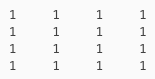
\includegraphics[scale=0.5]{images/pantalla1.png}
\end{center}
\end{column}
\end{columns}
\begin{exampleblock}{Comando}
Ver comando: zeros()
\end{exampleblock}
\begin{columns}
\begin{column}{0.5\textwidth}
Ej. Ejecutar las siguientes líneas. Obtener conclusiones.
\boiteviolette{
MatrizUnos = zeros(2,2)
}
\end{column}
\begin{column}{0.5\textwidth}
\begin{center}
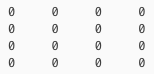
\includegraphics[scale=0.5]{images/pantalla2.png}
\end{center}
\end{column}
\end{columns}
\begin{block}{Tener en cuenta}
Cuando se usa una sola entrada, el resultado es una matriz cuadrada. Cuando se usan dos entradas, especifican el número de filas y columnas.
\end{block}
\end{frame}

\begin{frame}{Matrices especiales: Matriz identidad}
\begin{exampleblock}{Comando}
Ver comando: eye()
\end{exampleblock}
\begin{columns}
\begin{column}{0.5\textwidth}
Ej. Ejecutar las siguientes líneas. Obtener conclusiones.
\boiteviolette{
MatrizIdentidad = eye(3)
}
\end{column}
\begin{column}{0.5\textwidth}
\begin{center}
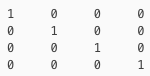
\includegraphics[scale=0.5]{images/pantalla3.png}
\end{center}
\end{column}
\end{columns}
\begin{block}{Tener en cuenta}
Cuando se usa una sola entrada, el resultado es una matriz cuadrada. Cuando se usan dos entradas, especifican el número de filas y columnas.
\end{block}
\end{frame}


%%%%%%%%%%%%%%%%%%%%%%%%%%%%%%%%%%%%%%%%%%%%%%%%%%%%%%%%%%%%%%%%%%%%%

% Sección de consultas

%%%%%%%%%%%%%%%%%%%%%%%%%%%%%%%%%%%%%%%%%%%%%%%%%%%%%%%%%%%%%%%%%%%%%

\section{Consultas}
\begin{frame}{Consultas}
\begin{center}

\includegraphics[scale=0.3]{images/consultas.png}
\end{center}
\end{frame}


%%%%%%%%%%%%%%%%%%%%%%%%%%%%%%%%%%%%%%%%%%%%%%%%%%%%%%%%%%%%%%%%%%%%%

% Sección de bibliografía

%%%%%%%%%%%%%%%%%%%%%%%%%%%%%%%%%%%%%%%%%%%%%%%%%%%%%%%%%%%%%%%%%%%%%

\section{Bibliografia}

\begin{frame}{Bibliografía}
\begin{columns}
\begin{column}{0.5\textwidth}
\begin{center}

\includegraphics[scale=0.4]{images/biblio1.png}
\end{center}
\end{column}
\begin{column}{0.5\textwidth}
\begin{center}
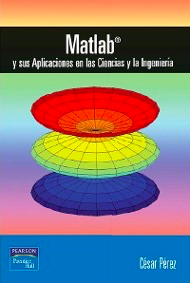
\includegraphics[scale=0.5]{images/biblio2.png}
\end{center}
\end{column}
\end{columns}
\end{frame}

\end{document}
